% Beamer do material do curso de Verão (2015) do IME-USP
% Introdução ao Projeto de Jogos
%
% Baseado no template LaTeX das apresentações do LIDET versão 2
% (https://github.com/luigivieira/LIDET)
%

\providecommand\classopts{}
\expandafter\documentclass\expandafter[table, usenames, svgnames, dvipsnames, \classopts]{beamer}

\usepackage{etex}
\usepackage{beamerthemeshadow}
\usepackage[portuguese]{babel}
\usepackage[utf8]{inputenc}
\usepackage[absolute,overlay]{textpos}
\usepackage{array}
\usepackage{framed}
\usepackage{booktabs}
\usepackage[compatibility=false]{caption}
\usepackage{subcaption}
\usepackage{outlines}
\usepackage{ulem}
\usepackage{xcolor,colortbl}
\usepackage{ragged2e}
\usepackage{tikz}

% ---------------------------------------------------------------------------- %
% Presentation definitions
% ---------------------------------------------------------------------------- %
\usetheme{Luebeck}
\hypersetup{pdfpagemode=FullScreen} % Starts the presentation in full screen

% layout
\setbeamerfont{frametitle}{size=\normalsize}
\setbeamerfont{title}{size=\normalsize}
\beamertemplatenavigationsymbolsempty
\setbeamertemplate{bibliography item}[text]%
\setbeamertemplate{headline}{} % Remove upper bar

% colors
\definecolor{lidet_orange}{rgb}{0.9, 0.49, 0.09}
\definecolor{lidet_black}{rgb}{0.2, 0.2, 0.2}

\setbeamercolor{title}{bg=lidet_orange}
\setbeamercolor{structure}{bg=white, fg=lidet_orange}
\setbeamercolor{normal text}{fg=black}
\setbeamercolor{section in head/foot}{fg=white, bg=lidet_black}
\setbeamercolor{postit}{fg=white, bg=lidet_orange!90!lidet_black}

% shadow
\makeatletter
\pgfdeclareverticalshading[black,bg]{bmb@shadow}{200cm}{%
  color(0bp)=(lidet_black!25); color(4bp)=(black!50!bg); color(8bp)=(black!50!bg)}
\pgfdeclareradialshading[black,bg]{bmb@shadowball}{\pgfpointorigin}{%
  color(0bp)=(black!50!bg); color(4bp)=(lidet_black!25)}
\pgfdeclareradialshading[black,bg]{bmb@shadowballlarge}{\pgfpointorigin}{%
  color(0bp)=(black!50!bg); color(4bp)=(black!50!bg); color(8bp)=(lidet_black!25)}
%
\makeatother

% Captions for images and tables
\setlength{\abovecaptionskip}{5pt plus 5pt minus 5pt}
\setlength{\belowcaptionskip}{5pt plus 5pt minus 5pt}
\captionsetup[figure]{font=scriptsize,labelfont=scriptsize}
\captionsetup[table]{font=scriptsize,labelfont=scriptsize}
\captionsetup{labelformat=empty,labelsep=none}

% Dimensions for table rules
\setlength\heavyrulewidth{0.1em} 
\setlength\lightrulewidth{0.01em}
\setlength\belowrulesep{0.10ex}
\setlength\aboverulesep{0.10ex}

% Define macros to mark the begining and ending of references
% Basically, handles the automatically spanned frames (due to parameter allowframebreaks)
% as backup frames, so they do not influence in the frame numbering
\newcommand{\referencesbegin}{
   \newcounter{framenumberappendix}
   \setcounter{framenumberappendix}{\value{framenumber}}
}
\newcommand{\referencesend}{
   \addtocounter{framenumberappendix}{-\value{framenumber}}
   \addtocounter{framenumber}{\value{framenumberappendix}} 
}

% Adjust footnotes to not overlap the footbar
\addtobeamertemplate{footnote}{}{\vspace{1.0ex}}
\let\oldfootnotesize\footnotesize
\renewcommand*{\footnotesize}{\oldfootnotesize\tiny}

% Redefine the quote environment so short quotes are not broken easily
\renewenvironment{quote}
	{\list{}{\leftmargin1em\rightmargin\leftmargin}%
	\item\relax}
	{\endlist}

% Section frames (that appear before each section)
\AtBeginSection[] 
{
	{
		\setbeamertemplate{footline}{} % Hide the footline locally for these frames
		\begin{frame}<beamer>[noframenumbering]
			\begin{center}
				\begin{tikzpicture}
					\node[align=left, left color=lidet_orange, right color=lidet_orange, draw, rounded corners, minimum width=10cm, minimum height=1cm] {\color{white} \textbf{\insertsectionhead}};
				\end{tikzpicture}
			\end{center}
			\footnotesize{ \tableofcontents[currentsection, hideothersubsections] }
		\end{frame}
	}
}

\AtBeginSubsection[]
{
    \begin{frame}
        \centering
        \Large
        \textbf{\insertsubsection}
    \end{frame}
}

\AtBeginSubsubsection[]
{
    \begin{frame}
        \centering
        \large
        \insertsubsection
        \vskip 1em
        \Large
        \textbf{\insertsubsubsection}
    \end{frame}
}

\DeclareGraphicsExtensions{.pdf,.jpg,.png}
\graphicspath{{./images/}}

% ---------------------------------------------------------------------------- %
% Presentation title, author and institution
% ---------------------------------------------------------------------------- %
\newcommand{\lessontitle}{Aula 4 - Pensando na Estética do Jogo}
\title{\textbf{Introdução ao Projeto de Jogos}}
\subtitle{{\small \lessontitle}}

\newcommand{\autores}{Luiz C. Vieira, Vinícius K. Daros}
\author[\autores]{\scriptsize
    Luiz Carlos Vieira e Vinícius Kiwi Daros\\
    \{luigivieira,vinicius.k.daros\}@gmail.com
}

\newcommand{\lidet}{LIDET (IME - USP)}
\institute[\lidet]{\\[1.0mm]
Curso de Verão (2015)\\
Departamento de Ciência da Computação}

\date{{\tiny 19 de Janeiro de 2016}}

% ---------------------------------------------------------------------------- %
% Presentation content
% ---------------------------------------------------------------------------- %

% ---------------------------------------------------------------------------- %
\begin{document}
% ---------------------------------------------------------------------------- %

% ---------------------------------------------------------------------------- %
% First Slide (index 0) = cover
% ---------------------------------------------------------------------------- %

{%\usebackgroundtemplate{}} 
\begin{frame}[plain, noframenumbering]

	\begin{columns}[c]
		\column{0.2\textwidth}
			\hspace*{-1.5em}
			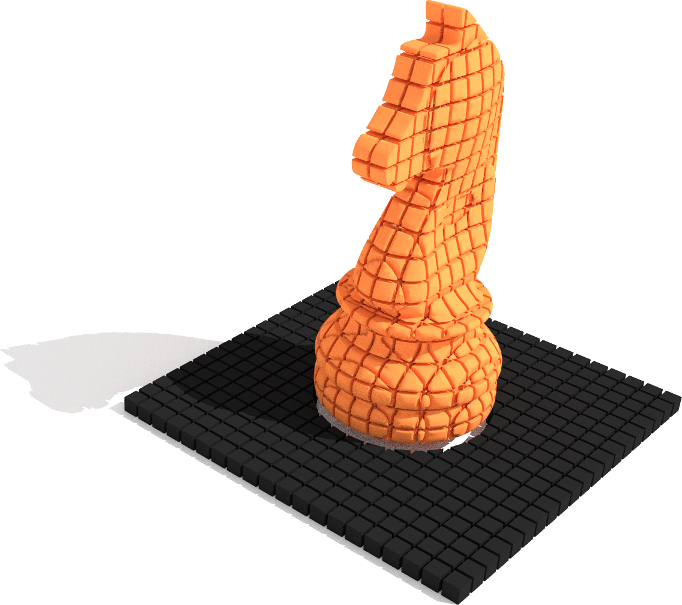
\includegraphics[width=0.35\paperwidth]{side_bar}\\
		\column{0.01\textwidth}
		\column{0.70\textwidth}
			\titlepage
			\hspace*{+0.5em}
			\begin{center}
				
\includegraphics[height=1.0cm]{lidet-logo}\\
				
\includegraphics[height=1.0cm]{ime-logo}\\
			\end{center}
	\end{columns}
	%\addtocounter{framenumber}{-1}
\end{frame}
}

% ---------------------------------------------------------------------------- %
% Other Slides (index from 1 onwards)
% ---------------------------------------------------------------------------- %

% setup navigation symbols and footline
\setbeamertemplate{navigation symbols}{}
\makeatletter
\setbeamertemplate{footline}{%
    \leavevmode%
    \hbox{%
        \begin{beamercolorbox}[wd=0.28\paperwidth,ht=4ex,dp=1ex,left,%
                               leftskip=2ex]{author in head/foot}%
            \usebeamerfont{title in head/foot}
            \insertdate\newline%
            \vskip 0.6ex%
            \autores
        \end{beamercolorbox}%
        \begin{beamercolorbox}[wd=0.53\paperwidth,ht=4ex,dp=1ex,center]%
                              {author in head/foot}%
            \usebeamerfont{author in head/foot}\lessontitle%
        \end{beamercolorbox}%
        \begin{beamercolorbox}[wd=0.19\paperwidth,ht=4ex,dp=1ex,right,%
                               rightskip=2ex]{author in head/foot}%
            \insertframenumber{}/\inserttotalframenumber \newline
            \lidet%
        \end{beamercolorbox}%
    }%
    \vskip 4cm%
}
\makeatother

% ---------------------------------------------------------------------------- %
\begin{frame}[plain]
\frametitle{\textbf{Agenda}}

	\hspace*{+4.0em}
	\footnotesize{ \tableofcontents }
\end{frame}

% ---------------------------------------------------------------------------- %
\section{Prazer sensorial (Juiciness)}
% ---------------------------------------------------------------------------- %

% ------------------------------
\begin{frame}{\textbf{O que é \textit{Juiciness}?}}
    \centering
    \begin{minipage}{8cm}
        \textit{Juiciness} são recompensas sensoriais que aumentam a impressão de
        que o jogo é vivo e responsivo. Se baseia em dar muito feedback mesmo para
        poucas ou pequenas ações.
        \vskip 1em

        Efeitos (visuais, sonoros, etc) que poderiam não existir, mas que existindo
        melhoram a experiência de jogo.
    \end{minipage}

\end{frame}

% ---------------------------------------------------------------------------- %
\section{Exemplos}
% ---------------------------------------------------------------------------- %

\subsection{Efeitos Sonoros}
% ------------------------------
\begin{frame}{\textbf{``Provocações'' automáticas}}
	\centering
	\begin{figure}
        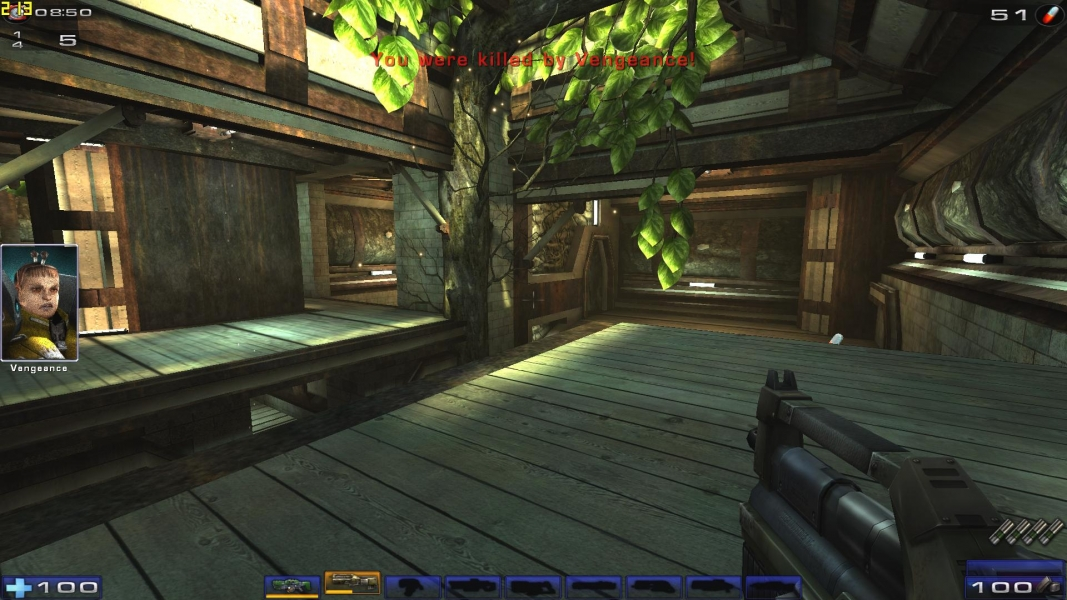
\includegraphics[height=5cm]{taunt}
        \caption{\scriptsize\textbf{Unreal Tournament 2004}\footnote{http://www.wsgf.org/f/u/imagecache/node-gallery-display/contrib/dr/247/ingame\_16x9.jpg}}
	\end{figure}
\end{frame}

\subsection{Movimento}
% ------------------------------
\begin{frame}{\textbf{Fruit Ninja}}
	\centering
	\begin{figure}
        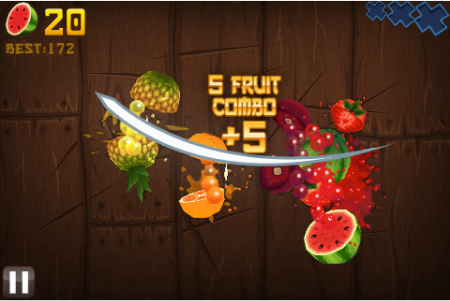
\includegraphics[height=5cm]{fruit_ninja}
        \caption{\scriptsize\textbf{Fruit Ninja}\footnote{http://upload.wikimedia.org/wikipedia/en/0/03/FruitNinja\_screenshot.png}}
	\end{figure}
\end{frame}

% ------------------------------
\begin{frame}{\textbf{Sonic derrapando}}
	\centering
    Vídeo 8
\end{frame}

\subsection{Luz}
% ------------------------------
\begin{frame}{\textbf{Luz guiando o jogador}}
	\centering
	\begin{figure}
        \begin{subfigure}{\textwidth}
        	\centering
            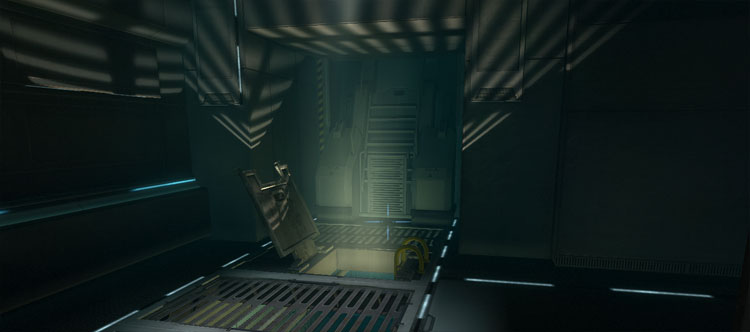
\includegraphics[height=2.7cm]{fear1}
            \caption{\scriptsize\textbf{F.E.A.R. 2}\footnotemark{}}
	    \end{subfigure}

        \begin{subfigure}{\textwidth}
	        \centering
            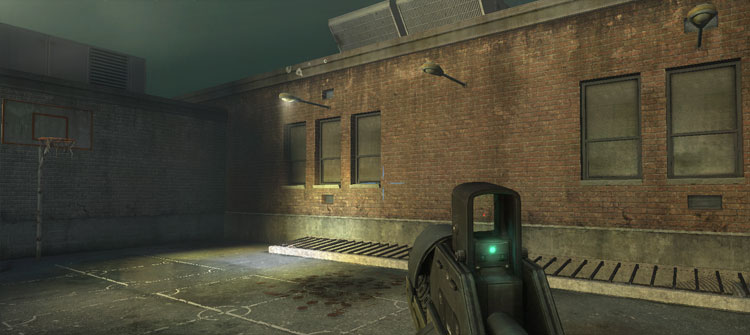
\includegraphics[height=2.7cm]{fear2}
            \caption{\scriptsize\textbf{F.E.A.R. 2}\footnotemark{}}
	    \end{subfigure}
	\end{figure}

	\footnotetext[1]{\url{http://www.clement-melendez.com/portfolio/articles/05/Fear2\_Light2.jpg}}
	\footnotetext{\url{http://www.clement-melendez.com/portfolio/articles/05/Fear2\_Door8.jpg}}
\end{frame}

%\subsection{Vitoria Espetacular}

%\subsection{Comportamento Viciante}

% ---------------------------------------------------------------------------- %
\subsection{Exemplos Comparativos}
% ---------------------------------------------------------------------------- %

% ------------------------------
\begin{frame}{\textbf{Bang! Bang! vs Worms}}

	\begin{figure}
	    \centering

	    \begin{subfigure}[!h]{0.4\paperwidth}
	    	\centering
	    	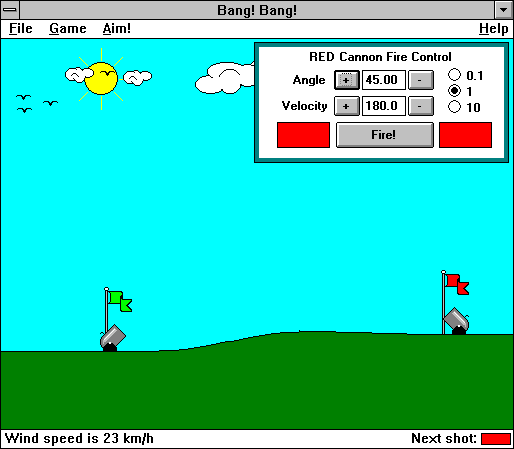
\includegraphics[height=0.4\paperheight]{bang_bang}
	        \caption{\scriptsize\textbf{Bang! Bang!}\footnotemark{}}
	    \end{subfigure}
	    ~
		\begin{subfigure}[!h]{0.4\paperwidth}
			\centering
	        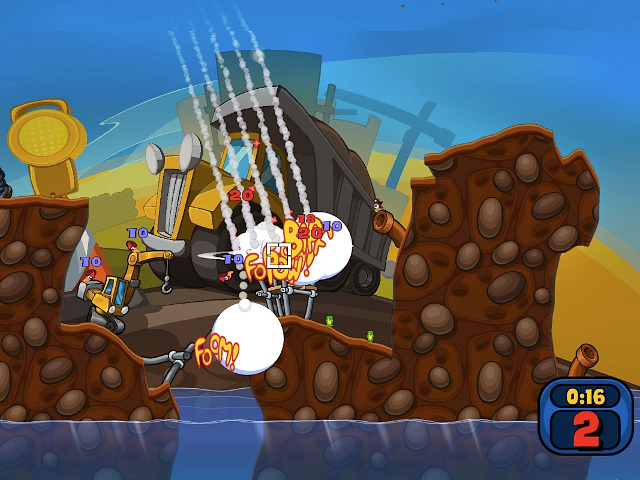
\includegraphics[height=0.4\paperheight]{worms}
	        \caption{\scriptsize\textbf{Worms Reloaded}\footnotemark{}}
	    \end{subfigure}
    \end{figure}

	\footnotetext[1]{\url{http://www.download-central.ws/Win16/Games/B/Bang!Bang!/screenshot.png}}
	\footnotetext{\url{http://www.blogcdn.com/www.joystiq.com/media/2010/07/wrair-strike.jpg}}

\end{frame}

% ------------------------------
\begin{frame}{\textbf{Crush the Castle vs Angry Birds}}

	\begin{figure}
	    \centering

	    \begin{subfigure}[!h]{0.4\paperwidth}
	    	\centering
	    	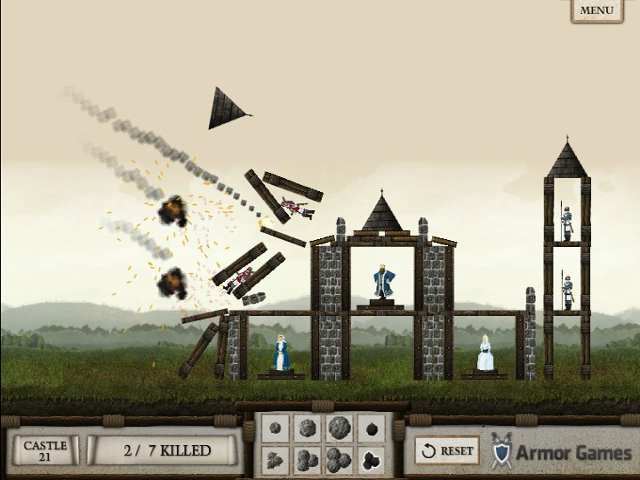
\includegraphics[height=0.4\paperheight]{crush-castle-screenshot}
	        \caption{\scriptsize\textbf{Crush the Castle}\\\copyright{2009} Armor Games\footnotemark{}}
	    \end{subfigure}
	    ~
		\begin{subfigure}[!h]{0.4\paperwidth}
			\centering
	        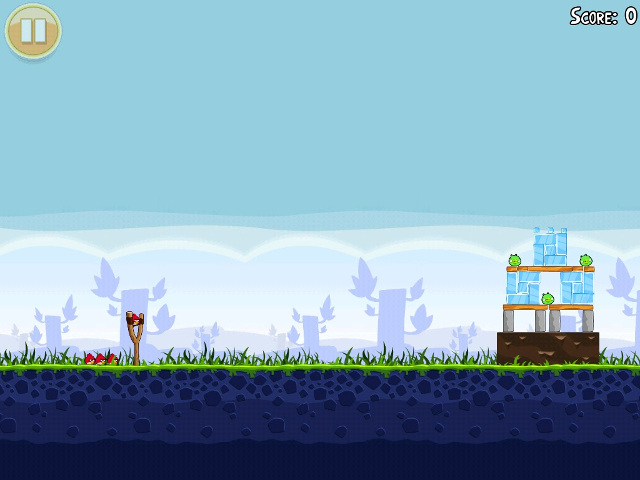
\includegraphics[height=0.4\paperheight]{angry-birds-screenshot}
	        \caption{\scriptsize\textbf{Angry Birds}\\\copyright{2009} Rovio\footnotemark{}}
	    \end{subfigure}
    \end{figure}

	\footnotetext[1]{\url{http://armorgames.com/play/3614/crush-the-castle/}}
	\footnotetext{\url{http://www.rovio.com/en/our-work/games/view/1/angry-birds/}}

\end{frame}

% ------------------------------
\begin{frame}{\textbf{Bejeweled 3 vs Candy Crush Saga}}

	\begin{figure}
	    \centering

	    \begin{subfigure}[!h]{0.4\paperwidth}
	    	\centering
	    	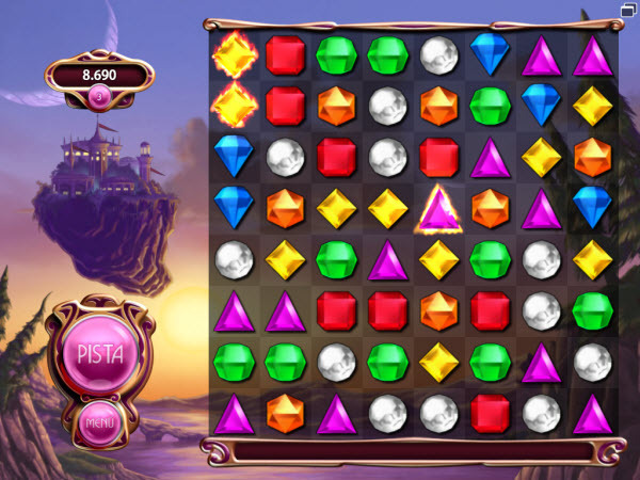
\includegraphics[height=0.4\paperheight]{bejeweled-screenshot}
	        \caption{\scriptsize\textbf{Bejeweled 3}\\\copyright{2010} PopCap Games\footnotemark{}}
	    \end{subfigure}
	    ~
		\begin{subfigure}[!h]{0.4\paperwidth}
			\centering
	        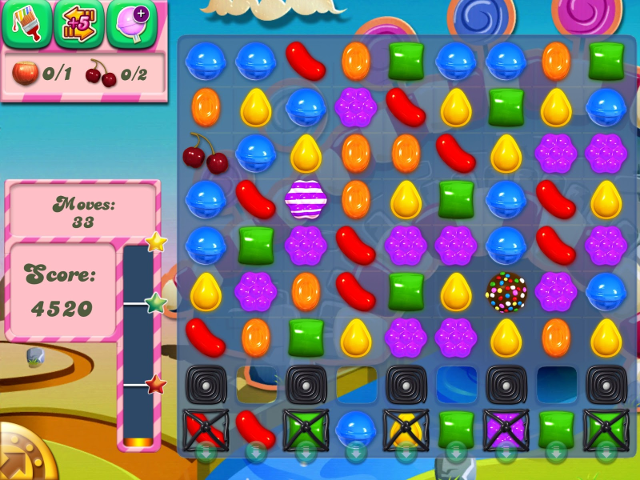
\includegraphics[height=0.4\paperheight]{candy-crush-screenshot}
	        \caption{\scriptsize\textbf{Candy Crush Saga}\\\copyright{2012} King\footnotemark{}}
	    \end{subfigure}
    \end{figure}

	\footnotetext[1]{\url{http://www.popcap.com/bejeweled-3/}}
	\footnotetext{\url{http://www.candycrushsaga.com/}}

\end{frame}

% ------------------------------
\begin{frame}{\textbf{Mercado de itens no Fallout e no Skirim}}

	\begin{figure}
	    \centering

	    \begin{subfigure}[!h]{0.4\paperwidth}
	    	\centering
	    	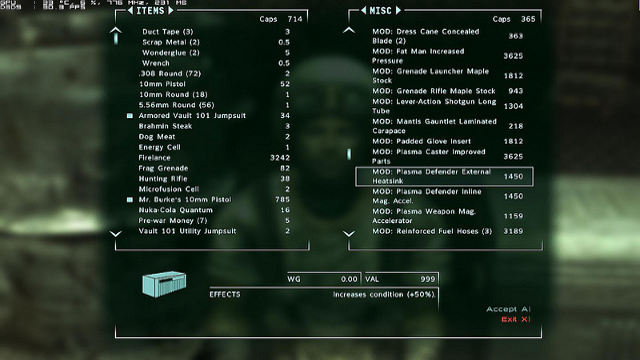
\includegraphics[height=0.32\paperheight]{fallout-screenshot}
	        \caption{\scriptsize\textbf{Fallout}\\\copyright{2008} Bathesda\footnotemark{}}
	    \end{subfigure}
	    ~
		\begin{subfigure}[!h]{0.4\paperwidth}
			\centering
	        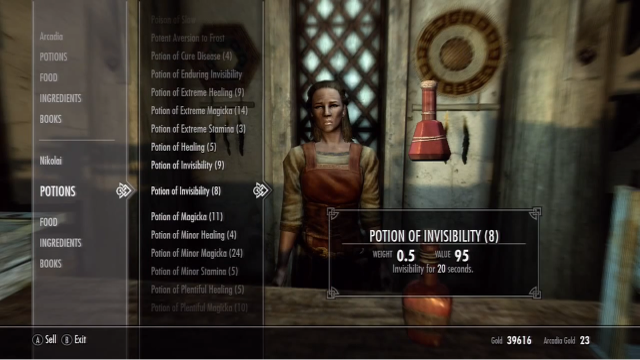
\includegraphics[height=0.32\paperheight]{skyrim-screenshot}
	        \caption{\scriptsize\textbf{The Elder Scrolls V: Skyrim}\\\copyright{2011} Bathesda\footnotemark{}}
	    \end{subfigure}
    \end{figure}

	\footnotetext[1]{\url{http://fallout.bethsoft.com/}}
	\footnotetext{\url{http://www.elderscrolls.com/skyrim/}}

\end{frame}

% ------------------------------
\begin{frame}{\textbf{Variações no porquinho do Angry Birds}}

	\begin{figure}
	    \centering

	    \begin{subfigure}[!h]{0.2\paperwidth}
	    	\centering
	    	
\includegraphics[height=0.2\paperheight]{angry-birds-pig1}
	        \caption{\scriptsize ao iniciar: em condição normal}
	    \end{subfigure}
	    ~
		\begin{subfigure}[!h]{0.2\paperwidth}
			\centering
	        
\includegraphics[height=0.2\paperheight]{angry-birds-pig2}
	        \caption{\scriptsize quase acertado: tensão e medo}
	    \end{subfigure}
	    ~
		\begin{subfigure}[!h]{0.2\paperwidth}
			\centering
	        
\includegraphics[height=0.2\paperheight]{angry-birds-pig3}
	        \caption{\scriptsize acertado: machucado}
	    \end{subfigure}
	    \\
		\begin{subfigure}[!h]{0.2\paperwidth}
			\centering
	        
\includegraphics[height=0.2\paperheight]{angry-birds-pig4}
	        \caption{\scriptsize acertado várias vezes: bem machucado}
	    \end{subfigure}
	    ~
		\begin{subfigure}[!h]{0.2\paperwidth}
			\centering
	        
\includegraphics[height=0.2\paperheight]{angry-birds-pig5}
	        \caption{\scriptsize falha total: risada irônica}
	    \end{subfigure}

	    \caption{\textbf{Os diferentes estados do porquinho de Angry Birds e a sensação transmitida}}
    \end{figure}

\end{frame}

% ---------------------------------------------------------------------------- %
\subsection{Juiciness como forma de controlar problemas}
% ---------------------------------------------------------------------------- %

% ------------------------------
\begin{frame}{\textbf{Evitando a parede invisível}}
    \centering
    Video 10
\end{frame}

% ------------------------------
\begin{frame}{\textbf{Efeitos sonoros para indicar eventos/estados}}
    \centering
    Video 11
\end{frame}

% ------------------------------
\begin{frame}{\textbf{Lidando com limitações técnicas}}
    \centering
    \begin{figure}
        
\includegraphics[height=5cm]{mario_original}
        \caption{\scriptsize\textbf{Mario}\footnote{https://hashtagus.files.wordpress.com/2013/11/super-mario-bros-original1.jpg?w=290}}
    \end{figure}
\end{frame}

% ---------------------------------------------------------------------------- %
\subsection{Mal uso do juiceness}
% ---------------------------------------------------------------------------- %

% ------------------------------
\begin{frame}{\textbf{Mal uso do juicenes}}
    \centering
    Animações longas e repetitivas

    \vskip 3em
    Vídeo 9
\end{frame}



% ---------------------------------------------------------------------------- %
\section{Prazer cognitivo não planejado}

% ------------------------------
\begin{frame}{\textbf{O bote mágico de Zork}}

\begin{columns}[c]  
\column{0.4\textwidth}
\begin{figure}
\centering

\includegraphics[height=0.5\paperheight]{zork}
\caption{\tiny \textbf{Zork I} \copyright{1980} Infocom\footnotemark{}}
\end{figure}
\column{0.6\textwidth}
\begin{outline}
\1 Nessa aventura de texto, o número de itens do inventário era limitado pelo peso total
\1 Um dos itens, um \textit{}, podia conter outros itens
\1 Ao ser desinflado, os itens desapareciam temporariamente (até o bote ser reinflado -- devido a um \textit{bug} de programação)
\2[-] {\scriptsize o jogador podia carregar um número muito maior de itens}
\1 Depois de descoberto, o erro não foi corrigido
\2[-] {\scriptsize o designer considerou que um jogador capaz de pensar nisso merecia usar o recurso!}
\end{outline}

\end{columns}
\footnotetext{\url{http://www.infocom-if.org/downloads/downloads.html}}
\end{frame}

% ------------------------------
\begin{frame}{\textbf{Battlefield 3}}
    \centering
    \begin{figure}
        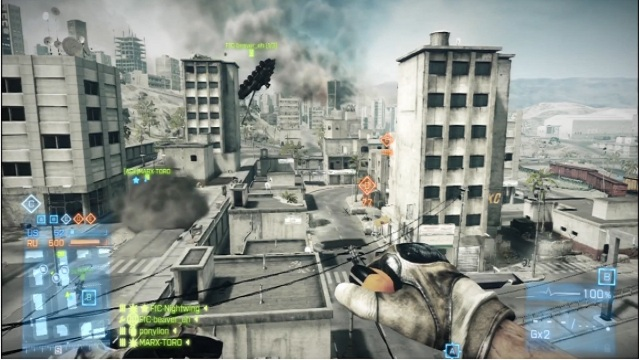
\includegraphics[height=5cm]{tank}
        \caption{\scriptsize\textbf{Battlefield 3}\footnote{http://d1vr6n66ssr06c.cloudfront.net/wp-content/uploads/2012/11/battlefield-3-flip.jpg}}
    \end{figure}
\end{frame}

\section{A Quarta Parede}

% ------------------------------
\begin{frame}{\textbf{Quebrando a quarta parede}}

	\begin{quotation}
		\noindent
		``Então, caso representeis, pensai no espectador apenas como se este não existisse. Imaginai, na borda do teatro, uma enorme parede que vos separe da plateia; representai como se a cortina não se levantasse''\\
		\hfill -- Denis Diderot (1713-1784)\\
		\hfill (filósofo e escritor Francês)\footnote{Fonte: \url{http://pt.wikipedia.org/wiki/Quarta_parede}}
	\end{quotation}
	
	\vspace{1em}

	\begin{outline}
		\1 O ato de ``derrubar a quarta parede'' tem origem na teoria do teatro
		
		\1 Refere-se a um personagem dirigindo sua atenção para a platéia
			\2[-] {\scriptsize ou tomando conhecimento de que os personagens e ações não são reais}
			
		\1 Tem efeitos humorísticos (nonsense) e de crítica
			\2[-] {\scriptsize já que intencionamente quebra a suspensão temporária de descrença}
	\end{outline}

\end{frame}

% ------------------------------
\begin{frame}{\textbf{As charadas do Charada}}

	\begin{figure}
		\centering
		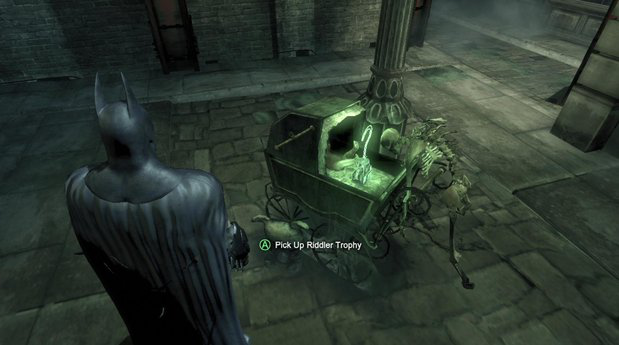
\includegraphics[height=0.3\paperheight]{batman-riddler}
		\caption{\tiny \textbf{Batman: Arkham Asylum} \copyright{2009} Warner Bros. Interactive\footnote{\url{http://www.warnerbros.com/videogame/batman-arkham-asylum}}}
	\end{figure}

	Após o jogador obter quase todos os troféus, o personagem Charada diz:

	\vspace{1em}

	\begin{verse}
		\noindent
		\Large
		``O quê? Quase completo? Você esta roubando? Procurou as respostas na Internet, não é?''\footnote{Tradução livre de: ``\textit{What? You're nearly done? Are you cheating? Looking them up on the internet? Tell me.}''}
	\end{verse}
	
	\vspace{1em}
	
\end{frame}

% ------------------------------
\begin{frame}{\textbf{As charadas do Charada}}

	\begin{figure}
		\centering
		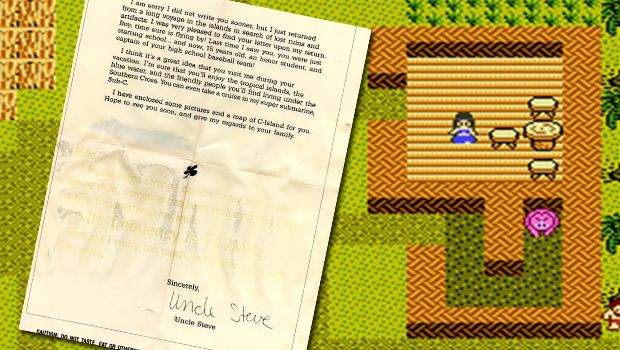
\includegraphics[height=0.3\paperheight]{startropics}
		\caption{\tiny \textbf{StarTropics} \copyright{1990} Nintendo\footnote{\url{http://www.nintendo.com/games/detail/mLqsyMiZqHleOYbtHCKqxhORw6JT45-g}}}
	\end{figure}

	\vspace{-1em}

	\begin{outline}
		\1 O manual do jogo acompanhava uma carta do tio do protagonista
			\2[-] {\scriptsize com informações relacionadas à fantasia, mas sem importância aparente}
			
		\vspace{1em}
		
		\1 Muito a frente no jogo, um personagem solicitava que a carta fosse mergulhada em água
			\2[-] {\scriptsize para obtenção de um código que permitiria a continuidade do jogo}
	\end{outline}

\end{frame}

% ------------------------------
\begin{frame}{\textbf{Leitor de mentes}}

	\begin{figure}
		\centering
		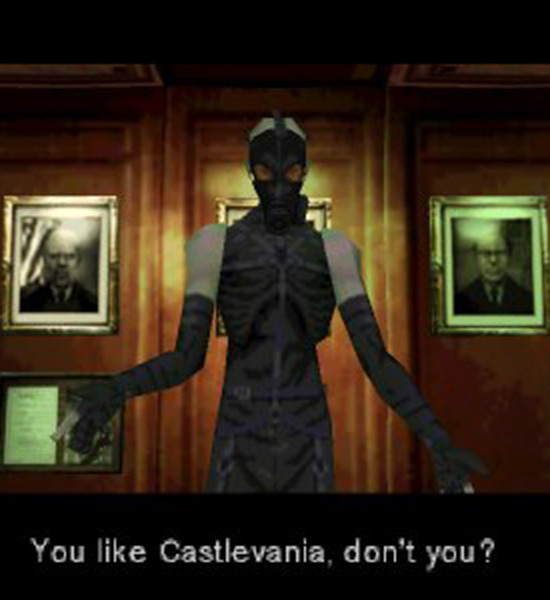
\includegraphics[height=0.4\paperheight]{metal-gear}
		\caption{\tiny \textbf{Metal Gear Solid} \copyright{1998} Konami\footnote{\url{https://www.konami.com/mgs/}}}
	\end{figure}

	\vspace{-1em}

	\begin{outline}
		\1 O vilão Psycho Mantis lia pensamentos
		
		\1 Citando jogos que o jogador gostava
			\2[-] {\scriptsize lendo dados de jogos gravados no cartão de memória}

		\1 Prevendo os golpes do jogador, de forma a ser impossível de vencer
			\2[-] {\scriptsize a não ser que o controle fosse conectado à outra porta do console}
	\end{outline}

\end{frame}

% ------------------------------
\begin{frame}{\textbf{Dezenas de outros exemplos}}

	\begin{outline}
		\1 Monkey Island 2: LeChuck's Revenge (1991)
			\2[-] {\scriptsize protagonista liga para desenvolvedors para criticar piada da versão anterior}
			
		\1 X-men (1993)
			\2[-] {\scriptsize para remover um vírus o jogador é solicitado a reiniciar o jogo}
									
		\1 Tomb Raider II (1997)
			\2[-] {\scriptsize protagonista está para tomar banho quando percebe o jogador assistindo}

		\1 Eternal Darkness: Sanity's Requiem (2002)
			\2[-] {\scriptsize perda de sanidade gera situações bizarras (simulação de sentar no controle remoto)}

		\1 Warcraft III: Reign of Chaos (2004)
			\2[-] {\scriptsize personagem é selecionado com o mouse e diz: ``Eu fui escolhido pela grande mão metálica no céu!''}

		\1 Assassin's Creed 2 (2009)
			\2[-] {\scriptsize personagem olha para o jogador e fala diretamente com ele}
			
		\1 The Stanley Parable (2013)
			\2[-] {\scriptsize narrador reconhece a insubordinação do jogador em seguir ordens}

	\end{outline}

\end{frame}

% ---------------------------------------------------------------------------- %
\section{Atividade}
% ---------------------------------------------------------------------------- %

% ------------------------------
\begin{frame}{\textbf{Atividade}}

	\begin{outline}
	
		\1 Descrever oportunidades de utilização de ``\textit{juiciness}'' em seu projeto
		
		\vspace{1em}
		
		\1 Atualizar sua documentação (GDD) conforme necessário
		
		\vspace{4em}

		\1 \textbf{OBSERVAÇÃO}: NÃO ESQUEÇAM DE TRAZER MATERIAL PARA A PROTOTIPAÇÃO NA PRÓXIMA AULA!
	
	\end{outline}

\end{frame}
\end{document}
